\documentclass[10pt]{article}

\usepackage{amsmath}
\usepackage{fullpage}
\usepackage{array}
\usepackage{graphicx}
\usepackage{gensymb}
\usepackage{booktabs}
\usepackage{gensymb}
\usepackage{graphicx}
\usepackage{hyperref}
\hypersetup{colorlinks,urlcolor=blue}


\graphicspath{ {../Images/} }

\date{2014-6-22}
\pagestyle{empty}
\setlength{\parindent}{0pt}

\begin{document}
\begin{center}
\begin{Large}\textbf{Chapter: Work Energy}\end{Large} \\
\smallskip
%\begin{large} Acceleration \end{large}
\end{center}
%%%%%%%
Objectives: Conservative forces, Potential energy (gravitational, spring), Conservation of mechanical energy.
\section{Potential energy}
Earlier in the class we learnt that there is an energy associated with the motion of the object known as kinetic energy.  In the last activity, we discovered that energy can be stored in the spring.  The amount of energy stored in the spring depends on the magnitude of the extension of the spring.  This energy is called potential energy.  For spring the potential energy is given by
\begin{equation}
  PE = \frac{1}{2}kx^2
\end{equation}
where $k$ is called the spring constant.  It follows from the Hooke's law which states that the force/tension developed in the string is \emph{lineraly} proportional to the extension in the spring.  It is given by
\begin{equation}
  F = -kx
\end{equation}
where $k$ is the spring constant and $x$ is the extension in the spring
\begin{figure}[h]
\label{springhooke}
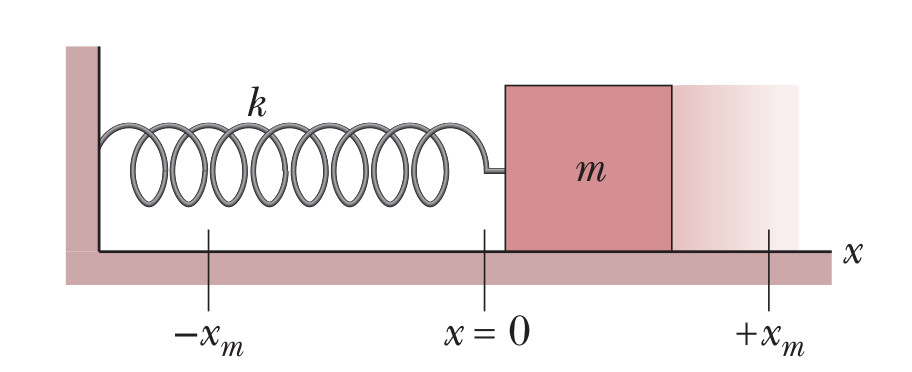
\includegraphics[scale=1]{springhooke}
\centering
\caption{Spring mass system}
\centering
\end{figure}
Note that the direction of the force is \emph{opposite} to that of the extension produced in the spring.

Now the $PE$ of the spring is only dependent on the initial and the final position of the mass (how?).  Such potentials are produced by the forces known as the \emph{conservative forces}.  Gravitational force is another example of a conservative force.  Therefore the potential energy associated with the objects in gravitational field should also depend only on the initial and final position of the mass.  

\begin{figure}[h]
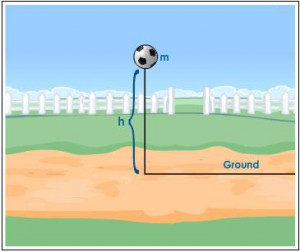
\includegraphics[scale=.5]{potenergyfootball}
\centering
\caption{Football at height $h$}
\label{potfootball}
\centering
\end{figure}
Consider a football tossed up at the height $h$ from the ground as shown in the figure \ref{potfootball}.  Then the potential energy of the football is given by the formula
\begin{equation}
  PE = mgh
\end{equation}
where $m$ is the mass of the football and $g$ is the acceleration due to gravity.
\section{Mechanical Energy}
The mechanical energy of the system is the linear sum of the potential energy and kinetic energy.  Symbolically
\begin{equation}
\begin{split}
  ME &= KE + PE\\
&= \frac{1}{2}mv^2 + mgx
\end{split}
\end{equation}
Now the law of the conservation of energy says that the total mechanical energy of the system is conserved in absence of the external force.  Actually this law is a consequence of a very beautiful theorem by \href{https://en.wikipedia.org/wiki/Emmy_Noether}{Emmy Noether} known as \href{https://en.wikipedia.org/wiki/Noether%27s_theorem}{Noether's Theorem}.  I would highly recommend reading the wikipedia page included in the hyperlink.  
\end{document}
